\documentclass[10pt,twocolumn,letterpaper]{article}

\usepackage{cvpr}
\usepackage{times}
\usepackage{epsfig}
\usepackage{graphicx}
\usepackage{amsmath}
\usepackage{amssymb}

% Include other packages here, before hyperref.

% If you comment hyperref and then uncomment it, you should delete
% egpaper.aux before re-running latex.  (Or just hit 'q' on the first latex
% run, let it finish, and you should be clear).
\usepackage[breaklinks=true,bookmarks=false]{hyperref}

\cvprfinalcopy % *** Uncomment this line for the final submission

\def\cvprPaperID{****} % *** Enter the CVPR Paper ID here
\def\httilde{\mbox{\tt\raisebox{-.5ex}{\symbol{126}}}}

% Pages are numbered in submission mode, and unnumbered in camera-ready
%\ifcvprfinal\pagestyle{empty}\fi
\setcounter{page}{4321}
\begin{document}

%%%%%%%%% TITLE
\title{Project: Car detection on KITTI dataset}

\author{Muhammad Haris Ibrahim\\
{\tt\small muhammad.ibrahim@student.uni-luebeck.de}
% For a paper whose authors are all at the same institution,
% omit the following lines up until the closing ``}''.
% Additional authors and addresses can be added with ``\and'',
% just like the second author.
% To save space, use either the email address or home page, not both
}

\maketitle
%\thispagestyle{empty}

%%%%%%%%% ABSTRACT
\begin{abstract}
  Detecting cars on the road is a critical task for autonomous driving. This must be done with high precision and in real-time. 
  In this paper, we develop a 2D car detector by fine tuning the YOLO-v3 object detector to detect cars on a scaled down version of KITTI dataset. 
  We achieved 50 percent mean Average Precision after finetuning YOLO-v3 model previously trained on MS COCO dataset. 
  Improvements to the training process are required to achieve better results.
\end{abstract}

%%%%%%%%% BODY TEXT
\section{Introduction}
Object detection is a critical task for autonomous driving. An autonomous vehicle must be able to detect and keep track of objects of interest in its environment. The classification of objects is not enough, their position and orientation in the environment must also be predicted. 
Another challenge is that these detections must be performed at high precision and recall but also in real-time on edge devices. The objects of interest can be lane line markings, traffic signs, vehicles, pedestrians and more. 

In this project, we focus only on detecting cars. Car detection is specially important in autonomous driving to avoid collisions and plan safe trajectories even at low levels of autonomy.

There are many deep learning based approaches for object detection. We adapt YOLO-v3 \cite{redmon2018yolov3}, a general purpose 2D object detector based on a Convolutional Neural Network (CNN) architecture. For training and evaluating our car detector, we will use a simplified version of KITTI dataset containing cars with 2D bounding box labels \cite{KITTI}.

YOLO-v3 is an improved version of YOLO \cite{redmon2016yolov1} which achieves 
higher mean Average Precision (mAP) on 2D object detection datasets like MS-COCO \cite{mscoco} while still being real-time. YOLO-v3 is a end to end CNN and performs predictions in only 1 pass.  

\begin{figure}[t]
	\begin{center}
		%\fbox{\rule{0pt}{2in} \rule{0.9\linewidth}{0pt}}
		\includegraphics[width=1.0\linewidth]{figure30.png}
	\end{center}
	\caption{Detections of the model developed in this project on a sample image from the test set.}
	\label{fig:pred_example_plot}
\end{figure}

Transfer learning is then used to finetune it for car detection on our version of KITTI dataset. We obtained 50 percent mean Average Precision (mAP) on a validation set.
%-------------------------------------------------------------------------
\section{Related Work}
Since the success of Convolutional Neural Network (CNN) based approaches like Alexnet \cite{Alexnet} on image classification tasks, many similar approaches have been designed for object detection. Region Proposal CNNs (RCNN) \cite{ren2015faster} and its various variants use handcrafted algorithms to generate proposals for regions of interest. These proposals are then passed to a CNN which produces class and confidence predictions. The predictions are then fed back into the region proposal algorithm. This means that multiple passes are required to perform good predictions. This makes these networks slow at inference time. These multi-stage detectors are, therefore, not realtime. 

YOLO architecture and Single Shot Detector \cite{SSD_v1} solved this problem by performing the object detection in only one evaluation of the network. These are end to end CNNs. Out of these two, YOLO is the fastest. 

YOLO architecture frames the object detection problem as a regression problem. It divides the image into a SxS grid, where S is the grid size. For each of these grid cells, there are three bounding box predictors in the output layer. A bounding box prediction consists of 4 coordinates of the bounding box. Each grid cell also includes a class prediction. 

YOLO-v3 also divides the images into SxS cell, but it produces class probabilities for each bounding box not just for each grid cell. Predictions are also made at three different scales. Prediction of the bounding box coordinates are also as offsets of bounding box priors (anchor boxes). These anchor boxes are based on shapes of bounding boxes common for the problem. The network outputs a large number of predictions. Bounding box and class predictions are made at 3 scales, SxS grid cells per scale, and 3 per grid cells. Non Maximum Suppression (NMS) is applied to keep only the best predictions. YOLO-v3 has already been applied to many object detection problems like face detection \cite{face_detection_yolo}, predestrian detection \cite{pedestrian_detection} and much more.

A brief comparison of the performance of many object detection frameworks in shown in Figure \ref {fig:detector_comparison}.

There are more recent and improved versions of YOLO such as \cite{yolov7} that are not developed by the original authors. Recent works like Detection Transformer \cite{DETR} use a CNN backbone with a transformer encoder and decode blocks. These approaches acheive higher mAP precision. They also remove the need for anchor boxes and NMS. Because of the limits of the dataset, limited time and GPU compute, we use the YOLOv3 architecture and not the newer ones.

\begin{figure}[t]
	\begin{center}
		%\fbox{\rule{0pt}{2in} \rule{0.9\linewidth}{0pt}}
		\includegraphics[width=1.0\linewidth]{object_detector_comparisons.png}
	\end{center}
	\caption{speed (ms) vs accuracy (AP) on MS. COCO test set. YOLOv3 outperforms many multistage and single stage object detectors in AP while being faster than all of them. This image is adapted from \cite{redmon2018yolov3} which is itself a version of image from \cite{retinaNet}}
	\label{fig:detector_comparison}
\end{figure}

\section{Method}
In this section, we provide a summary of the YOLO-v3 architecture.
\subsection{Bounding Boxes}
YOLO-v3 like many other object detectors does not predict the absolute coordinates of the bounding box. The bounding box centre coordinates are predicted as offsets to position of the top left corner of the grid cell. The width and height of the box are predicted as offset of the width and height of anchor boxes. These anchor boxes are pre-defined based on the likely shapes of anchor boxes for the problem at hand. The bounding box offsets are $t_x$, $t_y$, $t_w$, $t_h$. If the position of the top left of grid cell relative to the top left of the image is given by $(c_x, c_y)$ and the bounding box has width and height $p_w$, $p_h$, then the bounding box coordinates are calculated by: 
\begin{align*}
b_x &= \sigma(t_x) + c_x \\
b_y &= \sigma(t_y)  + c_y\\
b_w &= p_w e^{t_w}\\
b_h &= p_h e^{t_h}\\
\end{align*}
The ground truth values will be the left side of the above eqautions. We rearrange the equations to find the ground truth offsets.

The authors used clustering analysis to find the anchor box dimensions which have the most overlap with ground truth boxes on MS COCO dataset. We did not do such analysis on our dataset and used the anchor box dimensions reported in the orignal paper.

There are 09 anchors boxes---03 at each scale. Each grid cells within a scale, predicts three bounding boxes as offsets of these anchors boxes. The anchor boxes are in sets of three where the size of each set is according to the prediction scale.

\subsection{Objectness score}
Along with 04 coordinates of the bounding box, the network also predicts a objectness score for the bounding box. At test time, this is the confidence of the model in predicting that an object exists in the box and how well the box fits the object. At training time, this score should be the interesection over union between the predicted box and the ground truth box. The loss function forces this behaviour.

\subsection{Class predictions}
The network predicts a class probability for each bounding box. At training time, we use Cross entropy loss for classification prediction of the box. This is probality that there exists an object of class i given that there is an object in the box, $\Pr(\textrm{Class}_i | \textrm{Object})$. We can multiply this by objectness score to get the classification confidence.

\subsection{Features extraction backbone}
The backbone of the network is a 53 layer CNN named as Darknet 53. The overall summary of the layers is shown in Table \ref{network_architecture}. The authors did not explain any further details about the backbone. After spending sometime with the source code, our understanding is that each CNN block in the Table consists of a CNN layer, followed by leaky ReLU activation layer, and lastly a Batch Normalization layer. The filter sizes are mentioned in the Table. The 1x, 2x and such labels in the Table show the number of repeats. So, 2x means that such a block is repeated 2 times. It should be noted that the architecture includes skip connections like Resnets \cite{Resnets}. The authors trained this backbone for image classification on ImageNet dataset \cite{imagenet_dataset}. Further details about the training process is were not provided. We assume a strategy similar to the YOLO-v1 was used.

\subsection{Three Scale Predictions}
The extracted features of the backbone are then passed to the detection heads at three different scales. The size of the outputs are decided by dividing the image into SxS grid. There are three different grid sizes for three different scales. The idea is to use a coarses grid to help detect large object, then a medium size grid and then finally a smaller grid size. At each scale, the network has SxS predictors. Each grid cell has three predictors. Each predictor then predicts 4 bounding box coordinates (as offsets to three anchors), 1 objectness score and C class probabilities for C classes. So the total predictions at each scale are $S\times S\times [3*(4+1+C)]$. 
After the output of the feature extract backbone, several convolutional layers are added. The overall structure can be seen in Figure \ref{fig:detection_head}
The detection head for the first scale then adds two more Convolutional blocks. The outputs of this blocks is a $S\times S\times [3*(4+1+C)]$ tensor. 
For the second scale prediction, we take the output of the network just where the first detection head is attached and then upscale it by $2x$. We then concatenate this feature map with a feature map a couple of blocks before. The idea is to use earlier feature maps along with upscaled current feature maps to make predictions on a higher resolution. This helps with detecting medium and small objects. The second detection head is then attached here which then adds two more CNN blocks to make predictions. The process is repeated to get predictions for the third scale. 


\begin{figure}[t]
	\begin{center}
		%\fbox{\rule{0pt}{2in} \rule{0.9\linewidth}{0pt}}
		\includegraphics[width=1.0\linewidth]{detection_heads.png}
	\end{center}
	\caption{speed (ms) vs accuracy (AP) on MS. COCO test set. YOLOv3 outperforms many multistage and single stage object detectors in AP while being faster than all of them. This image is adapted from \cite{redmon2018yolov3} which is itself a version of image from \cite{retinaNet}}
	\label{fig:detection_head}
\end{figure}


\begin{table}[h] 
\begin{center}
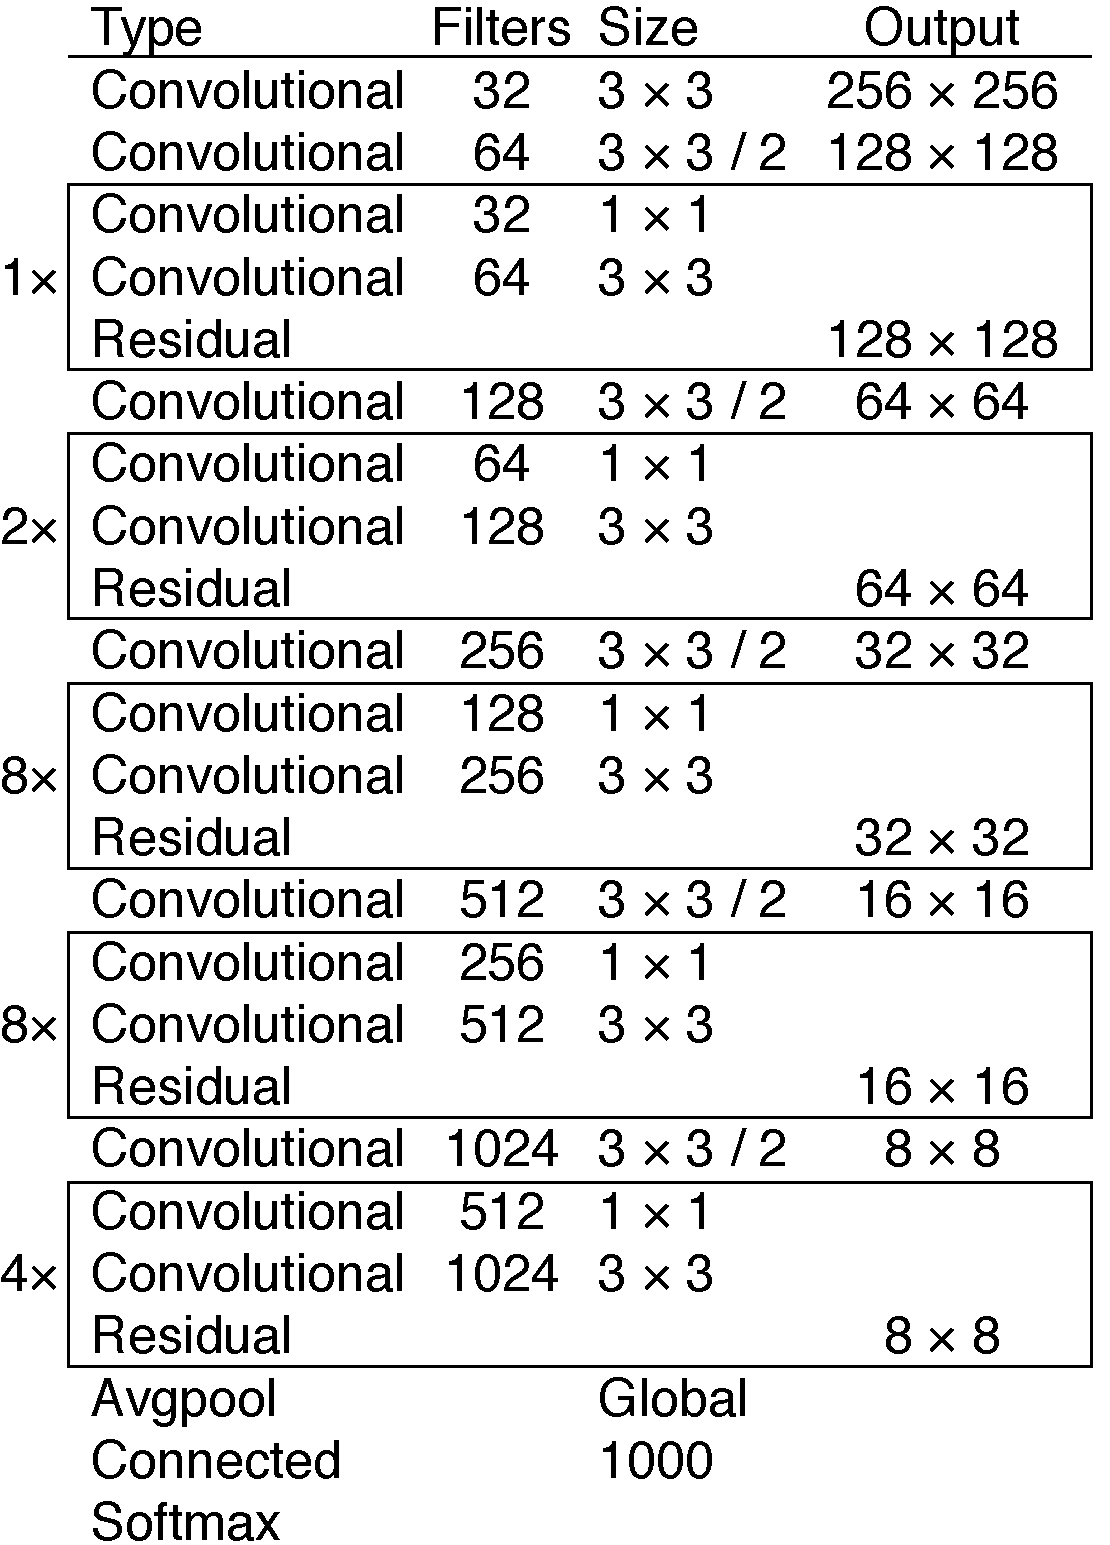
\includegraphics[width=.8\linewidth]{arch2.pdf}
\end{center}
\caption{\small \textbf{Darknet-53.}}
\label{network_architecture}
\end{table}

The network makes predictions at three different scales inspired by feature pyramid networksstage of the network


YOLO-v3 predicts 04 bounding box coordinates. These are the x and y coordinates for the centre of the box and width and height of the bounding box. The centre is predicted relative to the bounds of the grid cell edge. The equation for the bounding box look like:

On the left side are the absolute

They acheived this by dividing the image into a SxS grid of "predictors". Each predictor is responsible for generating predictions for an object, if the centre of the object bounding box lies in within the grid cell. The predictor generates a class probabilities, objectness confidence,
and 4 bounding box coordinates.

Also, formulas often help to make the mathematical background clearer. How to insert them is given here: 
$$a + b + a = 2 \cdot a + b\,.$$
It is essential that the reader is able to understand your method according to this section.

\section{Evaluation}
\subsection{Experimental Setup}
Here, you should describe the data you used for training, the hyper parameter settings, how you split the data into a training and a test set, etc.. Additionally, you should explain how you adapted your method to work well on your problem setup.




\subsection{Discussion}
In the discussion, you present and discuss the results your method achieved in the provided setups, why which set up works better, ... . The numbers (accuracy of your TEST set) should be given in a table, as e.g. Table \ref{tab:results}. You should also show exemplary images for which you achieved good results and examples, where the algorithm did not work as expected. Give possible explanations for both cases, e.g. ``what could be the reason for missing a Pedestrian? ``.

\begin{table}
	\begin{center}
		\begin{tabular}{|l|c|}
			\hline
			Method & Frobnability \\
			\hline\hline
			Theirs & Frumpy \\
			Ours & Makes one's heart Frob\\
			\hline
		\end{tabular}
	\end{center}
	\caption{Results. Ours is better.}
	\label{tab:results}
\end{table}

\section{Conclusion and Future Work}
Finally, you shortly summarize what you achieved in your work and point out what could be done in the future to get even better results. 









%-------------------------------------------------------------------------

{\small
\bibliographystyle{ieee_fullname}
\bibliography{literature}
}

\end{document}
